\documentclass[10pt,letterpaper]{article}
\usepackage[utf8]{inputenc}
\usepackage[T1]{fontenc}
\usepackage[margin=0.6in]{geometry}
\usepackage{amsmath,amssymb,mathtools,graphicx,booktabs,xcolor,hyperref}
\setlength{\parindent}{0pt}
\setlength{\parskip}{5pt}
\begin{document}

\section*{Block S2 Solutions: Wheatstone Bridge Analysis via KVL/KCL}

  \textbf{Companion Key to:} \texttt{Block\_S2\_Exercises\_Wheatstone\_Bridge.pdf} ~|~
  \textbf{Verification:} Cross-checked via Spec v2 Modified Nodal Analysis (MNA)


\subsection*{01 $\cdot$ Solutions: Null-Balance Condition \& Sensitivity Calculus Proof \hfill [10 Points]}


  \subsubsection*{(a) Null-Balance Proof from KCL \& KVL [4 points]}
  \textbf{(i) Node Potentials \& Leg Currents:} When $I_{LR} = 0$, Ohm's law across $R_G$ gives $V_L - V_R = I_{LR} R_G = 0 \implies V_L = V_R$. By KCL at node $L$, $I_1 = I_2 + I_{LR} = I_2$; by KCL at node $R$, $I_3 + I_{LR} = I_4 \implies I_3 = I_4$.
  \textbf{(ii) Ratio Proof:} Since $V_L = V_R$ and $V_B = 0\text{ V}$, the voltage drops across the upper resistors are equal ($V_T - V_L = V_T - V_R \implies I_1 R_1 = I_3 R_3$) and the voltage drops across the lower resistors are equal ($V_L = V_R \implies I_2 R_2 = I_4 R_4$). Dividing the first equation by the second and using $I_1 = I_2$, $I_3 = I_4$:
  $$\frac{I_1 R_1}{I_2 R_2} = \frac{I_3 R_3}{I_4 R_4} \implies \frac{R_1}{R_2} = \frac{R_3}{R_4} \Longleftrightarrow R_1 R_4 = R_2 R_3. \quad \blacksquare$$
  \textbf{(iii) Source \& Meter Independence:} Neither $V_T$ nor $R_G$ appears in $R_4 = \frac{R_2 R_3}{R_1}$ because both legs scale proportionally with $V_T$ ($V_L = \frac{R_2}{R_1+R_2}V_T$ and $V_R = \frac{R_4}{R_3+R_4}V_T$), so setting $V_L = V_R$ cancels $V_T$ completely (for any $V_T \neq 0$) and produces zero drop across any $R_G$.

  \subsubsection*{(b) Exact Unbalanced Bridge Current $I_{LR}(R_4)$ \& Sensitivity Derivative [6 points]}
  \textbf{(i) Closed-Form Formula [4 pts]:} Looking into node $L$ (with $R_G$ removed), the left voltage divider ($R_1 = 150\ \Omega, R_2 = 300\ \Omega$) has open-circuit voltage and Th\'evenin resistance:
  $$V_{\text{Th},L} = 15.0\left(\frac{300}{150 + 300}\right) = 10.0\text{ V}, \qquad R_{\text{Th},L} = \frac{(150)(300)}{150 + 300} = 100\ \Omega.$$
  Looking into node $R$, the right divider ($R_3 = 150\ \Omega$, variable $R_4$) has:
  $$V_{\text{Th},R}(R_4) = \frac{15.0 R_4}{150 + R_4}, \qquad R_{\text{Th},R}(R_4) = \frac{150 R_4}{150 + R_4}.$$
  Connecting $R_G = 100\ \Omega$ between $L$ and $R$ gives:
  $$I_{LR}(R_4) = \frac{V_{\text{Th},L} - V_{\text{Th},R}(R_4)}{R_{\text{Th},L} + R_G + R_{\text{Th},R}(R_4)} = \frac{10.0 - \frac{15.0 R_4}{150 + R_4}}{200 + \frac{150 R_4}{150 + R_4}} = \frac{1500 - 5.0 R_4}{30000 + 350 R_4} = \frac{300 - R_4}{6000 + 70 R_4}\text{ A} = \frac{300 - R_4}{6.00 + 0.0700 R_4}\text{ mA}.$$
  \textbf{(ii) Calculus Sensitivity at Balance [2 pts]:} Differentiating via the quotient rule:
  $$\frac{dI_{LR}}{dR_4} = \frac{(-1)(6000 + 70 R_4) - (300 - R_4)(70)}{(6000 + 70 R_4)^2} = \frac{-27000}{(6000 + 70 R_4)^2}\text{ A}/\Omega.$$
  Evaluating at $R_4 = 300\ \Omega$ ($6000 + 70(300) = 27000\ \Omega$):
  $$\left.\frac{dI_{LR}}{dR_4}\right|_{R_4 = 300\ \Omega} = -\frac{27000}{(27000)^2} = -\frac{1}{27000}\text{ A}/\Omega \approx -37.0\ \mu\text{A}/\Omega.$$

Final Key (Ex 01): ~ (a) $R_1/R_2 = R_3/R_4$ ~|~ (b) $I_{LR}(R_4) = \dfrac{300 - R_4}{6.00 + 0.0700 R_4}\text{ mA}$, ~ $\left.\dfrac{dI_{LR}}{dR_4}\right|_{300\ \Omega} = -37.0\ \mu\text{A}/\Omega$


\newpage



\subsection*{02 $\cdot$ Solutions: Unbalanced Wheatstone Bridge Nodal \& Mesh Analysis \hfill [14 Points]}


  \textbf{(a) Irreducibility [2 pts]:} Because node $L$ is a 3-way junction connecting $R_1, R_2$, and $R_G$ (with $I_{LR} \neq 0$), $R_1$ and $R_2$ do not carry the same current (not in series), and $R_1$ and $R_3$ do not share both terminal nodes because $R_G$ separates $L$ from $R$ (not in parallel).
  \textbf{(b) KCL \& KVL Equations [4 pts]:} With $V_T = 15.0\text{ V}$ and $V_B = 0\text{ V}$:
  \begin{itemize}
    \item \textbf{KCL at node $L$:} $\dfrac{V_L - 15.0}{150} + \dfrac{V_L - 0}{300} + \dfrac{V_L - V_R}{100} = 0 \xrightarrow{\times 300} 2(V_L - 15.0) + V_L + 3(V_L - V_R) = 0 \implies 6 V_L - 3 V_R = 30.0 \implies 2 V_L - V_R = 10.0$.
    \item \textbf{KCL at node $R$:} $\dfrac{V_R - 15.0}{150} + \dfrac{V_R - 0}{150} + \dfrac{V_R - V_L}{100} = 0 \xrightarrow{\times 300} 2(V_R - 15.0) + 2 V_R + 3(V_R - V_L) = 0 \implies -3 V_L + 7 V_R = 30.0$.
    \item \textbf{KVL around upper loop ($T \to L \to R \to T$):} $-150 I_1 - 100 I_{LR} + 150 I_3 = 0$.
  \end{itemize}
  \textbf{(c) Solving for $V_L, V_R$, and $I_{LR}$ [5 pts]:} From the first equation, $V_R = 2 V_L - 10.0$. Substituting into the second equation:
  $$-3 V_L + 7(2 V_L - 10.0) = 30.0 \implies 11 V_L = 100.0 \implies V_L = \frac{100}{11}\text{ V} \approx 9.09\text{ V}, \qquad V_R = \frac{90}{11}\text{ V} \approx 8.18\text{ V}.$$
  The signed bridge current from $L$ to $R$ is:
  $$I_{LR} = \frac{V_L - V_R}{R_G} = \frac{10/11\text{ V}}{100\ \Omega} = +\frac{1}{110}\text{ A} \approx +9.09\text{ mA}\text{ (flows from }L\text{ to }R\text{)}.$$
  \textbf{(d) All Leg Currents \& $R_{\text{eq}}$ [3 pts]:}
  $$I_1 = \frac{15 - 100/11}{150} = \frac{65/11}{150} = \frac{13}{330}\text{ A} \approx 39.4\text{ mA}, \qquad I_2 = \frac{100/11}{300} = \frac{1}{33}\text{ A} \approx 30.3\text{ mA},$$
  $$I_3 = \frac{15 - 90/11}{150} = \frac{75/11}{150} = \frac{1}{22}\text{ A} \approx 45.5\text{ mA}, \qquad I_4 = \frac{90/11}{150} = \frac{3}{55}\text{ A} \approx 54.5\text{ mA}.$$
  $$I_{\text{src}} = I_1 + I_3 = \frac{13}{330} + \frac{15}{330} = \frac{28}{330} = \frac{14}{165}\text{ A} \approx 84.8\text{ mA}, \qquad R_{\text{eq}} = \frac{15.0\text{ V}}{14/165\text{ A}} = \frac{2475}{14}\ \Omega \approx 177\ \Omega.$$

Final Key (Ex 02): ~ $V_L = 9.09\text{ V},\ V_R = 8.18\text{ V}$ ~|~ $I_{LR} = +9.09\text{ mA}$ ($L \to R$) ~|~ $I_{\text{src}} = 84.8\text{ mA},\ R_{\text{eq}} = 177\ \Omega$

\subsection*{03 $\cdot$ Solutions: Bridge Current Curve $I_{LR}(R_4)$ \& Conceptual Cloze \hfill [10 Points]}


  \textbf{Part A Landmark Values:} (1) $I_{LR}(0) = +50.0\text{ mA}$; (2) $I_{LR}(150\ \Omega) = +9.09\text{ mA}$; (3) $I_{LR}(300\ \Omega) = 0\text{ mA}$ (balanced); (4) $\lim_{R_4\to\infty} I_{LR}(R_4) = -\frac{1}{0.0700} = -14.3\text{ mA}$.
  \textbf{Part B Cloze Key:} (a) \texttt{zero}, \texttt{equal to}; (b) \texttt{$300\ \Omega$}; (c) \texttt{from $L$ to $R$}; (d) \texttt{from $R$ to $L$}; (e) \texttt{unchanged}; (f) \texttt{both an open and a short circuit}; (g) \texttt{Kirchhoff's junction rule}.

\begin{center}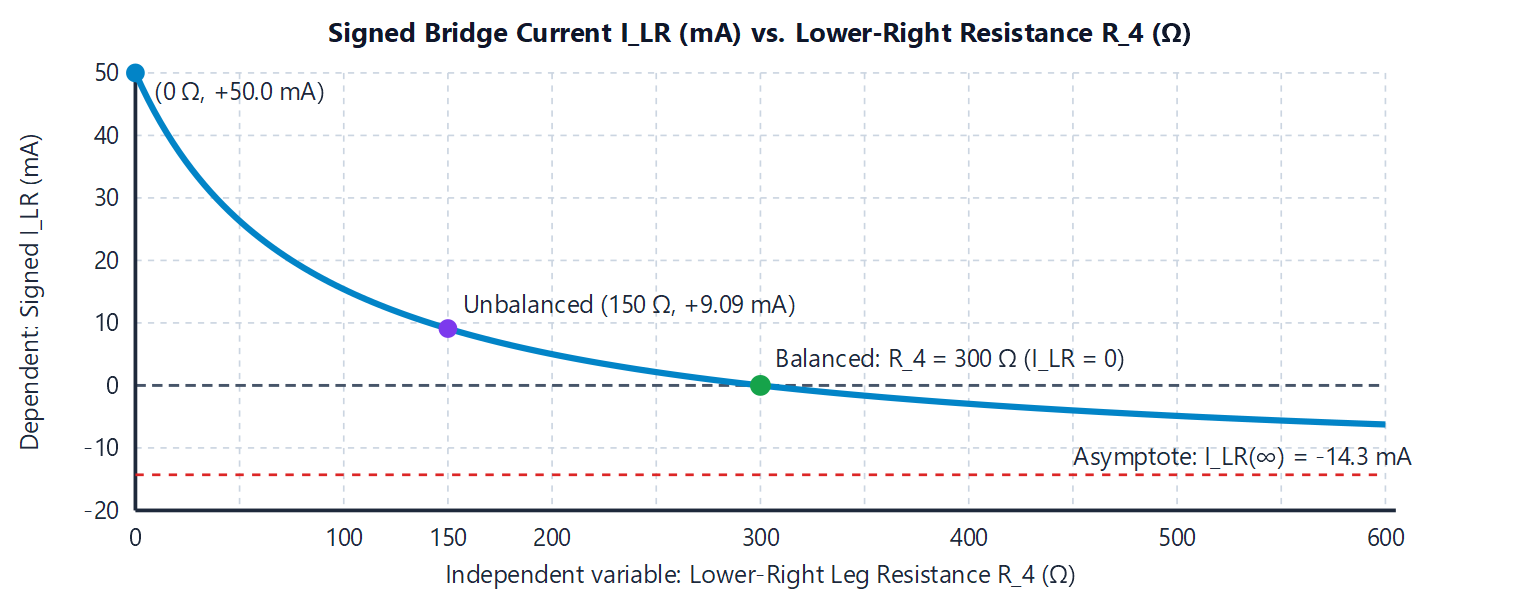
\includegraphics[width=0.82\linewidth]{day1_assets/s2-q3-grid-solved.png}\end{center}

\end{document}
